% This paper is part of the single transits project.
% Copyright 2015 Dan Foreman-Mackey (NYU) and the co-authors listed below.
%
%  RULES OF THE GAME
%
%  * 80 characters
%  * line breaks at the ends of sentences
%  * eqnarrys ONLY
%  * ``light curve'' not ``light-curve'' or ``lightcurve''
%  * Do not put in any comments that might get tweeted by @OverheardOnAph
%    (or maybe do put in a few....)
%  * ``percent'' (not \%) is a unit, as is ppm, so 5~percent.
%  * that is all.
%

\documentclass[12pt,preprint]{aastex}

\pdfoutput=1

\usepackage{color,hyperref}
\definecolor{linkcolor}{rgb}{0,0,0.5}
\hypersetup{colorlinks=true,linkcolor=linkcolor,citecolor=linkcolor,
            filecolor=linkcolor,urlcolor=linkcolor}
\usepackage{url}
\usepackage{amssymb,amsmath}
\usepackage{subfigure}
\usepackage{booktabs}

\usepackage{natbib}
\bibliographystyle{apj}

\newcommand{\project}[1]{\textsl{#1}}
\newcommand{\kepler}{\project{Kepler}}
\newcommand{\KT}{\project{K2}}
\newcommand{\tess}{\project{TESS}}
\newcommand{\jwst}{\project{JWST}}
\newcommand{\terra}{\project{TERRA}}
\newcommand{\pdc}{\project{PDC}}
\newcommand{\license}{MIT License}
\newcommand{\projectname}{\project{ketu}}

\newcommand{\paper}{\textsl{Article}}

\newcommand{\foreign}[1]{\emph{#1}}
\newcommand{\etal}{\foreign{et\,al.}}
\newcommand{\etc}{\foreign{etc.}}
\newcommand{\True}{\foreign{True}}
\newcommand{\Truth}{\foreign{Truth}}

\newcommand{\figref}[1]{\ref{fig:#1}}
\newcommand{\Fig}[1]{\figurename~\figref{#1}}
\newcommand{\fig}[1]{\Fig{#1}}
\newcommand{\figlabel}[1]{\label{fig:#1}}
\newcommand{\Tab}[1]{Table~\ref{tab:#1}}
\newcommand{\tab}[1]{\Tab{#1}}
\newcommand{\tablabel}[1]{\label{tab:#1}}
\renewcommand{\eqref}[1]{\ref{eq:#1}}
\newcommand{\Eq}[1]{Equation~(\eqref{#1})}
\newcommand{\eq}[1]{\Eq{#1}}
\newcommand{\eqalt}[1]{Equation~\eqref{#1}}
\newcommand{\eqlabel}[1]{\label{eq:#1}}
\newcommand{\sectionname}{Section}
\newcommand{\Sect}[1]{\sectionname~\ref{sect:#1}}
\newcommand{\sect}[1]{\Sect{#1}}
\newcommand{\sectalt}[1]{\ref{sect:#1}}
\newcommand{\App}[1]{Appendix~\ref{sect:#1}}
\newcommand{\app}[1]{\App{#1}}
\newcommand{\sectlabel}[1]{\label{sect:#1}}

\newcommand{\BIC}{{\ensuremath{\mathrm{BIC}}}}
\newcommand{\TIC}{{\ensuremath{\mathrm{TIC}}}}
\newcommand{\T}{\ensuremath{\mathrm{T}}}
\newcommand{\dd}{\ensuremath{\,\mathrm{d}}}
\newcommand{\bvec}[1]{{\ensuremath{\boldsymbol{#1}}}}
\newcommand{\appropto}{\mathrel{\vcenter{
  \offinterlineskip\halign{\hfil$##$\cr
    \propto\cr\noalign{\kern2pt}\sim\cr\noalign{\kern-2pt}}}}}
\newcommand{\densityunit}{{\ensuremath{\mathrm{nat}^{-2}}}}

% TO DOS
\newcommand{\todo}[3]{{\color{#2}\emph{#1}: #3}}
\newcommand{\dfmtodo}[1]{\todo{DFM}{red}{#1}}
\newcommand{\hoggtodo}[1]{\todo{HOGG}{blue}{#1}}

% Notation for this paper.
\newcommand{\period}{{\ensuremath{P}}}
\newcommand{\rp}{{\ensuremath{R_\mathrm{P}}}}
\newcommand{\rate}{{\ensuremath{\Gamma}}}

\newcommand{\datareleaseurl}{{\url{http://bbq.dfm.io/ketu}}}

\begin{document}

\title{%
    Searching for long-period transiting planets in the \kepler\ light curves
    using supervised classification
}

\newcommand{\nyu}{2}
\newcommand{\cds}{3}
\newcommand{\mpia}{4}
\newcommand{\mpis}{5}
\author{%
    Daniel~Foreman-Mackey\altaffilmark{1,\nyu,\cds},
    David~W.~Hogg\altaffilmark{\nyu,\mpia,\cds},
    Bernhard~Sch\"olkopf\altaffilmark{\mpis},
    \etal
}
\altaffiltext{1}         {To whom correspondence should be addressed:
                          \url{danfm@nyu.edu}}
\altaffiltext{\nyu}      {Center for Cosmology and Particle Physics,
                          Department of Physics, New York University,
                          4 Washington Place, New York, NY, 10003, USA}
\altaffiltext{\cds}      {Center for Data Science, New York University,
                          726 Broadway, 7th Floor, New York, NY, 10003, USA}
\altaffiltext{\mpia}     {Max-Planck-Institut f\"ur Astronomie,
                          K\"onigstuhl 17, D-69117 Heidelberg, Germany}
\altaffiltext{\mpis}     {Max Planck Institute for Intelligent Systems
                          Spemannstrasse 38, 72076 T\"ubingen, Germany}

\begin{abstract}

Many of the most dynamically interesting planets will be on orbits longer
than the baseline of existing transit surveys (\kepler, \KT).
Future surveys (\tess, PLATO?) will have such a short continuous coverage that
even habitable zone planets around M-dwarfs will only present a single transit
signal.
Searches for these transiting planets are plagued by false
signals---especially when pushed to low signal-to-noise---and statistical
studies of their population are complicated by weak constraints on the
physical parameters of the system and high rates of false positives.
We develop and present a computationally expensive but tractable method of
searching for single transits using supervised classification methods from
the machine learning literature.
For each month of photometry, we train a random forest classifier on a large
number of simulated signals injected into the photometry of the same star at
different times.
Then, the model's prediction as a function of transit time is evaluated and
times above a threshold probability---chosen for each star to yield a sample
with $\sim99$~percent purity---are given as candidate transits.
Each candidate must then pass a final round of vetting including BLAH BLAH
BLAH.
Applied to every light curve in the \kepler\ archive this method yields a
list of XXXX long-period transiting planet candidates.
Using an informative prior on their eccentricities, we derive weak constraints
on the orbital periods of the candidates and demonstrate that this puts an
upper limit of ZZZZ on the occurrence rate of these planets.

\end{abstract}

\keywords{%
methods: data analysis
---
methods: statistical
---
catalogs
---
planetary systems
---
stars: statistics
}

\section{Introduction}

\begin{itemize}

\item Description of the physical significance of these planets

\item Discussion of previous attempts (papers by Gaudi, Yee, Payne, Bakos,
\etc).

\item Comparison of method to filtering methods and an argument for why
supervised classification should be more robust to false alarms given a large
enough training set

\end{itemize}

\section{Estimated yield}

Before the launch of the \kepler\ Mission, \citet{Yee:2008} predicted the
yield of single transit events based on the planet occurrence rates estimated
based on small catalog of radial velocity discoveries \citep{Butler:2006} and
a fit to their occurrence rate \citep{Cumming:2008}.
Using these early results and the pre-launch specifications of the \kepler\
Mission, \citet{Yee:2008} predicted that \kepler\ would discover $\sim 6$
single transit events in the full dataset.
Now that the Mission is complete and we have better estimates of the
occurrence rate and distribution of planets \citep[for example][]{Dong:2013,
Petigura:2013, Foreman-Mackey:2014, Dressing:2015}, we can update the
predicted yield for single transit events in the \kepler\ light curves.
To make this estimate, we extrapolate the distribution of large planets on
relatively short orbits out to longer periods, taking detection efficiency
and the survey and targeting properties into account.

We will base our estimate on an assumed model $Q_k(\rp,\,\period)$ for the
absolute probability of detecting a planet with radius \rp\ and period
\period\ orbiting the star $k$, and the occurrence rate distribution
\begin{eqnarray}
\rate (\rp,\,\period) &=& \frac{\dd N}{\dd\ln\rp\dd\ln\period} \quad,
\end{eqnarray}
the expected number of planets per star, per logarithmic radius, per
logarithmic period.
Given these two quantities, the expected number of single transits in the
\kepler\ data is given by
\begin{eqnarray}
N &=& \sum_{k=1}^K N_k
\end{eqnarray}
where the sum is over the $K$ stars in the sample and $N_k$ is the expected
number of observable transits around star $k$
\begin{eqnarray}\eqlabel{nk}
N_k &=& \int Q_k(\rp,\,\period) \, \rate (\rp,\,\period)
    \dd\ln\rp \dd\ln\period \quad.
\end{eqnarray}
The integral in \eq{nk} is over the full range of target parameters.

For the purposes of this discussion, we assume an approximate simple detection
efficiency model with three contributions: the geometric transit probability,
the temporal transit probability, and signal-to-noise ratio threshold of the
search technique.
Assuming circular orbits, the geometric transit probability is given by
\citep{Winn:2010}
\begin{eqnarray}\eqlabel{q-geom}
Q_k^\mathrm{(geom)}(\rp,\,\period) &=& \frac{R_k}{a} \\
&=& \left( \frac{4\,\pi^2}{G\,M_k} \right)^{1/3} \, R_k \, \period^{-2/3}
\end{eqnarray}
where $R_k$ and $M_k$ are the radius and mass of the star $k$ respectively.
The eccentricity distribution of these long-period planets will affect this
transit probability \citep{Kipping:2014} but this simple prescription should
be sufficient for a rough estimate.
For long-period orbits, the temporal transit probability will be given by
\begin{eqnarray}\eqlabel{q-time}
Q_k^\mathrm{(time)}(\rp,\,\period) &=& \frac{T_k}{\period}
\end{eqnarray}
where $T_k$ is the total time that \kepler\ spent observing the star $k$.
Finally, the detection threshold depends on the detailed sensitivity of the
search procedure but we will approximate it as a simple step function in
signal-to-noise ratio of the transit.
This contribution will be given approximately by
\begin{eqnarray}
Q_k^\mathrm{(detect)}(\rp,\,\period) &=& \left\{\begin{array}{ll}
1 & \mathrm{if}\,\left(\rp/R_k\right)^2 > f\,\sigma_k \\
0 & \mathrm{otherwise}
\end{array}\right.
\end{eqnarray}
where $\sigma_k$ is an estimate of the noise in light curve of star $k$ and
$f$ is the detection threshold for the method.

Combining the detection efficiency components, the integral from \eq{nk}
becomes
\begin{eqnarray}\eqlabel{nk-2}
N_k &=& \left( \frac{4\,\pi^2}{G\,M_k} \right)^{1/3} \, R_k \, T_k
    \int_{\rp_\mathrm{min}} ^{\rp_\mathrm{max}} \frac{\dd\rp}{\rp}
    \int_{\period_\mathrm{min}} ^{\period_\mathrm{max}}
        \period^{-8/3}\,\rate(\rp,\,\period) \dd\period
\end{eqnarray}
where all the integration limits are set by the target parameter space.
Because of the detection probability threshold, $\rp_\mathrm{min}$ can be no
smaller than $R_k\,\sqrt{f\,\sigma_k}$.
\citet{Dong:2013} used the catalog of short period transiting planets found
by \kepler\ to constrain a model for the occurrence rate of large planets of
the form
\begin{eqnarray}
\rate(\rp,\,\period) &=& C\,\left(\frac{\period}{10\,\mathrm{d}}\right)^\beta
\end{eqnarray}
in a set of radius bins.
Using this model, the integral in \eq{nk-2} becomes
\begin{eqnarray}
N_k &=& \left( \frac{4\,\pi^2}{G\,M_k} \right)^{1/3} \, R_k \, T_k \,
    \sum_{j=1}^J \frac{C_j}{(10\,\mathrm{d})^{\beta_j}}\,
    \ln \left( \frac{\rp_{\mathrm{max},j}}{\rp_{\mathrm{min},j}} \right) \,
    \left[ \frac{{\period_\mathrm{min}}^{\beta_j - 5/3}}{5/3-\beta_j} \right]
\end{eqnarray}
where the sum is over the $J$ radial bins studied by \citet{Dong:2013}.
It's important to note that the model used by \citet{Dong:2013} is given in
base-10 logarithms so the units must be converted to natural logarithms as
appropriate.

Assuming the stellar parameters provided by the NASA Exoplanet
Archive\footnote{\dfmtodo{URL for kepler stellar table; downloaded on SOME
DATE.}} \dfmtodo{cite Huber} and approximating the stellar noise using the
15-hour CDPP \dfmtodo{cite CDPP}, \dfmtodo{some figure} shows the extrapolated
number of transiting planets with $\period > 1500\,\mathrm{d}$ based on the
\citet{Dong:2013} power-law model.
For a detection threshold $f\sim10$, the expected number of single transit
events in the \kepler\ light curves is $\sim 150$.

This results is much more optimistic than the pre-launch estimate from
\citet{Yee:2008} for a few reasons.
One effect is that, the \kepler\ Mission ran for more than four
years---longer than the fiducial Mission goal---and $\sim190,000$ stars were
targeted for nearly the full baseline instead of the original 100,000.
\dfmtodo{Explain other reasons.}

\begin{figure}[p]
\begin{center}
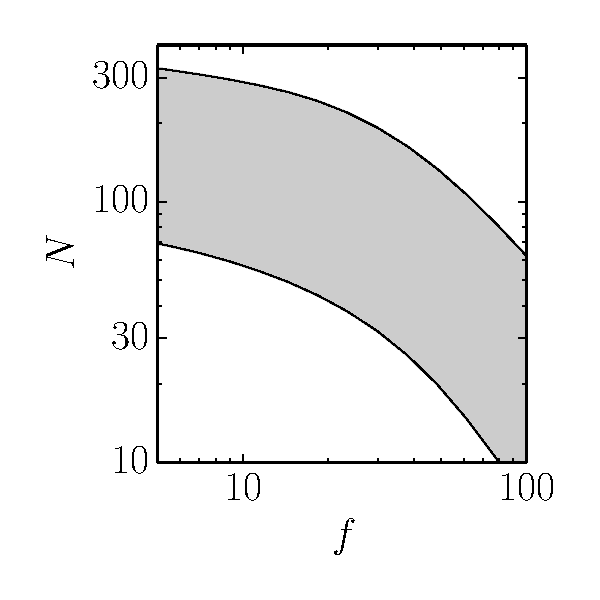
\includegraphics{figures/predict.pdf}
\end{center}
\caption{%
The expected number of single transit events---extrapolated from the
\citet{Dong:2013} power-law model fit to the shorter period \kepler\
candidates---as a function of the effective signal-to-noise threshold of the
search procedure.
The shaded region indicates the uncertainties propagated from the model
parameters.
\figlabel{predict}}
\end{figure}


\section{Data preparation}

The \kepler\ Mission measured photometry for about 190,000 stars at half-hour
cadence for a baseline of over four years.
We aim to search these time series for single transits of long-period planets
and single eclipses of binary stars.
These data are made available on
MAST\footnote{\url{https://archive.stsci.edu/kepler/}} and, for each target,
we downloaded the full set of light curve files provided by Data Release 24
\citep{Thompson:2015}.
From these files, we extracted the PDC time series and split them into
``sections'' with no more than two contiguous missing or flagged data points.
The PDC light curves have been corrected for the instrumental effects caused
by the spacecraft using a data-driven model of the focal plane
\citep{Stumpe:2012, Smith:2012}.
Crucially, an attempt is also made by the PDC procedure to remove sharp
instrumental artifacts like ``sudden pixel sensitivity dropouts (SPSDs)''.

The goal of this project is to discover the transits of long-period planets
that have not yet been discovered.
Therefore, when studying the light curve of an eclipsing binary star or a star
with known transiting planet candidates---on shorter periods---we also remove
all the in-transit data for the candidate using the parameters provided by the
\project{NASA Exoplanet
Archive}\footnote{\url{http://exoplanetarchive.ipac.caltech.edu/}; We
downloaded the \texttt{cumulative} table of \kepler\ Objects of Interest on
2015-03-25.}.

\paragraph{Terminology}

Any remaining missing data points are filled in using linear interpolation
resulting in sections of contiguous time series measurements with nearly
uniform time sampling.
This procedure yields about 150 \emph{light curve sections} for the typical
\kepler\ target.

As we discuss further below, a key assumption of our analysis is that the
process generating any non-transit variability or noise in the light curve
is stationary.

Every three months, the \kepler\ spacecraft rolled 90~degrees to maintain its
orientation with respect to the Sun.
This means that each star landed on a different set of pixels each quarter
and, therefore, the systematic signals caused by any specific spacecraft
orientation won't be shared between neighboring quarters.
A year later, however, the pointing would return to nearly the same setup and
each star ends up back on many of the same pixels.
This manifests itself in the light curves by causing the observations
separated by a year to be qualitatively similar.

For reasons that will become clear in \sect{search}, we split the light curve
sections into 3 disjoint sets.
We use these sets to run a train/validate/test procedure so the goal is to
have representative samples in each set.
Therefore, we attempt to split the sections intelligently; evenly
distributing sections from the same quarter and season across the splits.
When this is not possible, we randomly assign the section to a split.


\section{Random forest classification}

A common task in the machine learning literature is called \emph{supervised
classification} where the goal is to separate objects into classes
represented by sets of labeled examples.
One example from the astronomy literature is the problem of star--galaxy
separation (\dfmtodo{cite}).
In this problem, there are a set of images or photometric measurements that
have been classified---by some other method---as either a star or galaxy
observation and the goal is to transfer these labels to a set of observations
that have not yet been classified.
For a more in-depth discussion of the application of these techniques in
astronomy, the interested reader is directed to \citet{Ivezic:2013}.

The Random Forest (RF) classification model \citep{Breiman:2001} has become
very popular in the machine learning community.
It has also been applied with great success in astronomy \citep[for
example]{Richards:2011, Richards:2012} \dfmtodo{others}.
The RF model works by fitting an ensemble of decision trees to randomly
selected subsamples of the training dataset.
Each tree in the forest is ``grown'' by greedily choosing decision boundaries
that optimize the separation of the training data in randomly selected
subsets of the features until the separation is complete, each leaf contains
only one class or, at most, a fixed number of samples.
At each branch, the decision boundary is set by maximizing either the entropy
or the ``gini'' coefficient.

For the problem of single transit search, our problem can be phrased as a
classification problem where we want to assign every $K$ data point long chunk
of light curve into either the \texttt{transit} or \texttt{no transit} class.
This problem doesn't fall under the standard format of a supervised
classification problem because very few long-period transits have actually
been observed or classified.
We do think, however, that we have a good physical generative model for the
signal of interest and most of the observations of each star have no transits.
Therefore, we can train the model on simulated signals.

We use the \project{scikit-learn}\citep{Pedregosa:2011} implementation of the
RF classification algorithm\footnote{Specifically we use the
\texttt{RandomForestClassifier} object;
\url{http://scikit-learn.org/stable/modules/generated/sklearn.ensemble.RandomForestClassifier.html}.}.


\section{Search procedure}\sectlabel{search}

To search for single transits in the light curve of a specific star, we fit
three random forest models.

\paragraph{Generate the training \& validation sets}

We need to train the classification model on simulated signals.
To simulate these training and validation examples, we randomly select
sections of 121 contiguous flux measurements and simulate the transit signal
induced by the physical orbit of a large planet.
The specific distribution of simulated parameters is listed in \dfmtodo{some
table}.
In the simulations, we take limb darkening and integration time into account
\dfmtodo{cite}.
Since we expect most of the systematic variability to be time-reversible, we
augment the training set with simulations injected into the reversed time
series \dfmtodo{cite some examples of rotational invariance}.
The training set also includes an equal number of negative examples---time
series chunks of the same length without a simulated transit injection.
By virtue of the fact that we are specifically searching for single transits
it is safe to assume that none of the negative samples from the other light
curve sections will have no transits.

We also generate a validation set of simulated signals.
This set is identical to the training set except it is simulated in sections
of light curve that are not used for training.
As discussed below, this set is used to determine the transit significance
threshold required to achieve a pure sample.

In practice, we only need to train three models on the three disjoint
training sets and then for each model, we validate and test on both of the
remaining splits.


\paragraph{Features}

In many supervised classification problems, a sophisticated feature
extraction method is used to improve the performance of the procedure.
For this specific problem, we find excellent performance using the 121
normalized flux values as the features.
The depth of the transit and the noise in the light curve is not irrelevant
to detection so we don't normalize the features to unit variance in the
standard way.
Instead, we normalize each sample (feature vector) by it's empirical median
value and take the logarithm.
Another option for a feature set could be the Fourier transform or wavelet
transform of the light curve section.
Alternatively, the spectrogram of the fluxes in a larger window.
We have experimented briefly with this options finding similar performance.


\paragraph{Train}




\paragraph{Validate}

\paragraph{Test}


\section{Tuning parameters}\sectlabel{tuning}

Many choices need to be made in building this classification model.
These choices can be specified by a set of parameters that can be tuned the
optimize the performance of the method.
At this point, it's probably worth discussing how one might specifically
measure the ``performance'' of a search for transits.
The goal is, of course, to \emph{find transiting planets}.
Therefore, we would like to develop a method that finds the most planets
possible.
This will, in general, trade off with the purity of the sample.
For example, a method that returns every possible point the light curve as a
planet candidate will be guaranteed to find every signal in the dataset---it
will have excellent completeness or \emph{recall}---but almost every
candidate will be false---the \emph{precision} is low.
This is obviously not what we want.
Instead, the more relevant metric is probably the recall at fixed (high)
precision.

Let's be clear about what we mean by the terms \emph{precision} and
\emph{recall} in this context because they have specific definitions in the
machine learning that will be useful in our discussion here.
Recall is the probability, integrated across the full parameter space of
interest that a true transit signal will be detected by the method.
In astronomy, this quantity is generally called the completeness or the
detection efficiency and it is routinely measured for transit surveys
\dfmtodo{cite}.
On the other hand, precision is the probability that a positive classification
will be true.
In other words, for a given candidate that our pipeline spits out, the
probability that it is a false alarm is given by one minus the precision.
In astronomy, precision is generally hard or impossible to measure because we
have no ground truth; we don't know that \emph{there is definitely no transit}
at a given time in the light curve.
However, with a few weak assumptions, we can, in practice, estimate the
precision of our single transit search robustly.

\paragraph{Estimating the survey precision}

There are two key assumptions that enter into our precision calculation.
The first is that all transiting planets with more than one transit and a
large signal-to-noise ratio have been previously discovered by one of the many
transit searches applied the \kepler\ dataset \dfmtodo{cite}.
This is a safe assumption because, for large planets, these surveys are all
largely complete out to periods yielding only 2 or 3 transits in the \kepler\
baseline \dfmtodo{cite}.
The second necessary assumption is less robust but it is required for a
completely reliable measurement of the survey precision.
This assumption is that the noise processes in the data are stationary.
In other words, the transit-like noise signals in the training and validation
sets must be ``similar'' to the signals in the target section.
The PDC processing of the data successfully removes most of the
instrument-induced signals with some exceptions that are discussed in
\sect{demo}.
Perhaps we make the further assumption that the stellar variability is
also stationary.

Under these assumptions, the precision of the search procedure is
estimated using a set of injections.


\paragraph{The parameters}

\paragraph{Objective function}


\section{Preliminary results}\sectlabel{demo}

\paragraph{A discovery}



\paragraph{Successes}

\paragraph{Failures}


\section{Parameter estimation}

Even though only one transit is observed, it is still possible to estimate the
orbital period of these planet candidates using independent constraints on the
stellar properties.
This technique is similar in spirit to the ``photoeccentric effect''
\citep{Dawson:2012} and ``asterodensity profiling'' \citep{Kipping:2012}.
The fundamental principle is that, the transit duration is a measurement of
the instantaneous velocity of the planetary motion and this yields a
constraint on the orbital period when combining this with a measurement of the
stellar density and a prior on the eccentricity of the orbit.

In practice, we directly model the light curve as being generated by a planet
on an eccentric Keplerian orbit transiting a limb darkened star and
marginalize over all the orbital elements and physical parameters.
We take limb darkening and the finite exposure time into account
\citep{Mandel:2002, Kipping:2010, Kipping:2013} and use an empirical
Beta function prior on the eccentricity \citep{Kipping:2013a}.


\section{Population inference}

Based on our single transit discoveries, we now want to place a limit on
the occurrence rate of long-period planets.
Since we only have one discovery thus far, we'll make the simplifying
assumption that the rate is flat in log-period and log-radius in the range
$1000\,\mathrm{d} < \period < 5000\,\mathrm{d}$ and $5\,R_\odot <
20\,R_\odot$.
For this distribution, \citet{Foreman-Mackey:2014} derived the analytic
maximum likelihood result
\begin{eqnarray}
\rate &=& \frac{N_\mathrm{obs}}{\int Q(w)\dd w}
\end{eqnarray}
where $\rate$ is the occurrence rate per natural logarithm in period and
radius, $N_\mathrm{obs}$ is the number of detections, and the integral is over
the completeness measurements for every star that has been searched.
If we make the simplifying assumption that the detectability of a transit
depends on period only through Equations~(\eqref{q-geom})
and~(\eqref{q-time}), then this integral becomes
\begin{eqnarray}
\int Q(w)\dd w &=& \sum_{k=1}^K
    \left( \frac{4\,\pi^2}{G\,M_k} \right)^{1/3} \, R_k \, T_k \, Q_k \,
    \int \period^{-8/3}\,\rp^{-1} \dd\rp\dd\period \\
 &=& \sum_{k=1}^K
    \left( \frac{4\,\pi^2}{G\,M_k} \right)^{1/3} \, R_k \, T_k \, Q_k \,
    \ln \left(\frac{\rp_\mathrm{max}}{\rp_\mathrm{min}}\right)
    \frac{3}{5} \,
    \left[{\period_\mathrm{min}}^{-5/3} - {\period_\mathrm{max}}^{-5/3}\right]
\end{eqnarray}
where the sum is over all the targeted stars.

\section{Results}


\section{Discussion}


\acknowledgments
It is a pleasure to thank
\ldots
for helpful contributions to the ideas and code presented here.
DFM and DWH were partially supported by the National Science Foundation
(grant IIS-1124794),
the National Aeronautics and Space Administration
(grant NNX12AI50G), and the Moore--Sloan Data Science Environment at NYU.

This research made use of the NASA \project{Astrophysics Data System} and the
NASA Exoplanet Archive.
The Archive is operated by the California Institute of Technology, under
contract with NASA under the Exoplanet Exploration Program.
This \paper\ includes data collected by the \kepler\ mission. Funding for the
\kepler\ mission is provided by the NASA Science Mission directorate.
We are grateful to the entire \kepler\ team, past and present.
Their tireless efforts were all essential to the tremendous success of the mission
and the successes of \KT, present and future.
These data were obtained from the Mikulski Archive for Space Telescopes
(MAST).
STScI is operated by the Association of Universities for Research in
Astronomy, Inc., under NASA contract NAS5-26555.
Support for MAST is provided by the NASA Office of Space Science via grant
NNX13AC07G and by other grants and contracts.

{\it Facilities:} \facility{Kepler}

\appendix

\section{Some appendix}

\clearpage
\bibliography{peerless}
\clearpage


% \begin{figure}[p]
% \begin{center}
% \includegraphics{figures/pca.pdf}
% \end{center}
% \caption{%
% The top 10 eigen light curves (ELCs) generated by running principal component
% analysis on all the aperture photometry from Campaign~1.
% \figlabel{pca}}
% \end{figure}

\end{document}
